\documentclass[conference]{IEEEtran}
\usepackage{cite}
\usepackage{amsmath,amssymb,amsfonts}
\usepackage{algorithmic}
\usepackage{graphicx}
\usepackage{textcomp}
\usepackage{xcolor}
\usepackage{booktabs}
\usepackage{multirow}
\usepackage[hidelinks]{hyperref}

\def\BibTeX{{\rm B\kern-.05em{\sc i\kern-.025em b}\kern-.08em
    T\kern-.1667em\lower.7ex\hbox{E}\kern-.125emX}}

\begin{document}

\title{Deep Learning Meets Traditional Heuristics: A Neural Network-Augmented AI System for Mastering the Bavarian Card Game Schafkopf}

\author{\IEEEauthorblockN{Anonymous Author}
\IEEEauthorblockA{\textit{Department of Computer Science} \\
\textit{University Name}\\
City, Country \\
email@example.com}}

\maketitle

\begin{abstract}
We present a novel hybrid artificial intelligence system for developing game-playing agents that outperform traditional rule-based systems in the German trick-taking card game Schafkopf. Card games with incomplete information and dynamic team structures represent a significant challenge for machine learning approaches, requiring agents to reason under uncertainty while coordinating with unknown partners. While previous approaches using pure deep reinforcement learning methods such as Proximal Policy Optimization (PPO) and various supervised learning techniques failed to surpass a strong rule-based baseline, our innovative method leverages Monte Carlo simulation to generate oracle training data that systematically identifies suboptimal decisions in the rule-based agent. We introduce a novel pairwise ranking neural network model trained on 64,333 action pairs extracted from 43,420 game states, achieving 68.9\% ranking accuracy on held-out validation data. The resulting hybrid AI agent, which intelligently and selectively overrides the rule-based agent's decisions only when the neural ranking model exhibits high confidence, achieves a 57.7\% win rate against the baseline—a statistically significant 9 percentage point improvement with $p < 0.0001$. Our research demonstrates that learning to identify and correct specific weaknesses in existing heuristic systems can be substantially more effective than attempting to learn optimal play from scratch using end-to-end deep learning approaches. This methodology has broad implications for AI systems in domains where strong hand-crafted solutions already exist.
\end{abstract}

\begin{IEEEkeywords}
Schafkopf, card games, artificial intelligence, hybrid AI agents, Monte Carlo methods, deep neural networks, learning to rank, game-playing AI, reinforcement learning, decision-making systems
\end{IEEEkeywords}

\section{Introduction}

Card games have long served as challenging and compelling benchmarks for artificial intelligence research, dating from early foundational work on Poker \cite{billings2002challenge} to more recent groundbreaking advances in Bridge \cite{tian2020joint}. These games combine incomplete information, stochastic elements, and the critical need for strategic reasoning under uncertainty, making them particularly interesting and demanding testbeds for evaluating AI systems. The inherent complexity of card games—where agents must reason about hidden information, predict opponent behavior, and plan multiple moves ahead—provides an ideal proving ground for advancing the state of the art in machine learning and artificial intelligence.

Schafkopf is a traditional Bavarian trick-taking card game with unique characteristics that distinguish it from more commonly studied games in the AI literature. Unlike Poker, which has received extensive attention from the research community, Schafkopf features dynamic team formation where a solo player (known as the declarer) competes against three defenders, with one defender potentially serving as a hidden partner whose identity is revealed only through gameplay. The game uses a 32-card German deck with a complex and hierarchical trump ordering system, requiring agents to reason about card distributions, team coordination strategies, and sophisticated strategic card play. These characteristics make Schafkopf an excellent benchmark for studying AI in cooperative-competitive settings with imperfect information.

The challenge of developing strong AI agents for Schafkopf extends beyond simple card playing. Agents must simultaneously track played cards, infer the likely holdings of other players, coordinate with potential partners (whose identity may be unknown), and make decisions that balance immediate tactical considerations with longer-term strategic goals. This multi-faceted decision-making process under uncertainty represents a significant challenge for both traditional AI approaches and modern deep learning methods.

While rule-based approaches have been successfully applied to Schafkopf \cite{doppelkopf2019}, achieving strong play through carefully hand-crafted heuristics developed over years of expert analysis, such systems inevitably contain suboptimal patterns and decision-making weaknesses that exploit-aware opponents could potentially leverage. These rule-based systems, while generally effective, lack the ability to adapt to novel situations or learn from experience. Conversely, end-to-end deep learning approaches face the significant challenge of navigating a vast state space with sparse and delayed rewards, often failing to match rule-based performance within reasonable computational training budgets.

In this paper, we propose a novel hybrid approach that strategically combines the strengths of both paradigms while mitigating their respective weaknesses. Our key insight is that rather than learning to play optimally from scratch—a daunting task given the complexity of the game—we can use Monte Carlo simulation as an oracle to systematically identify situations where the rule-based agent makes suboptimal decisions. We then train a neural network to recognize similar situations during actual gameplay. The hybrid agent defaults to reliable rule-based play but intelligently overrides decisions when the learned model is confident that a demonstrably better action exists.

Our contributions are as follows:
\begin{itemize}
    \item A PettingZoo-compatible Schafkopf environment implementation with configurable game modes, enabling reproducible AI research on this underexplored game
    \item A Monte Carlo oracle method for generating ground-truth action values that reveal weaknesses in heuristic agents
    \item A novel pairwise ranking neural network architecture specifically designed for learning action preferences in card games
    \item Comprehensive empirical demonstration of a 57.7\% win rate against a strong rule-based baseline, representing a statistically significant improvement
    \item Analysis of when and how the neural network corrects rule-based decisions, providing insights into the nature of heuristic weaknesses
\end{itemize}

\section{Background}

\subsection{Schafkopf Rules and Game Mechanics}

Schafkopf is played with four players using a 32-card German deck consisting of four suits (Acorn, Leaf, Heart, Bell) and eight ranks (7, 8, 9, 10, Unter, Ober, King, Ace). The game has deep historical roots in Bavarian culture and represents one of the most strategically complex trick-taking card games in the European tradition. In the standard ``Sauspiel'' (partner game) mode, which is the focus of our research, the declarer calls an Ace of a non-trump suit, and the holder of that Ace becomes the declarer's partner—critically, this partnership remains unknown to other players until the called Ace is played, introducing an element of hidden information that significantly complicates strategic reasoning.

The trump hierarchy in Schafkopf is distinctive and more complex than in many other trick-taking games. All Obers (Queens) and Unters (Jacks) are permanent trumps regardless of their suit, ranked in the following strict order: Ober-Acorn $>$ Ober-Leaf $>$ Ober-Heart $>$ Ober-Bell $>$ Unter-Acorn $>$ Unter-Leaf $>$ Unter-Heart $>$ Unter-Bell. Additionally, Hearts serve as the trump suit, giving a total of 14 trump cards. Non-trump suits follow the standard order: Ace $>$ 10 $>$ King $>$ 9 $>$ 8 $>$ 7. This hierarchical structure creates complex strategic considerations about when to play trumps and how to manage trump resources throughout the game.

Card points are distributed as follows: Ace=11, 10=10, King=4, Ober=3, Unter=2, and all other cards carry zero points, totaling 120 points across all cards. The declarer team wins if they capture at least 61 points through won tricks. This point-based victory condition, combined with the asymmetric team structure and hidden partnership, creates a rich strategic landscape that has challenged human players for centuries.

\subsection{Related Work}

\subsubsection{Game-Playing Artificial Intelligence}
Deep reinforcement learning has achieved remarkable superhuman performance in various games, including the landmark achievements in Go \cite{silver2016mastering}, Chess and Shogi \cite{silver2017mastering}, and heads-up no-limit Texas Hold'em Poker \cite{brown2019superhuman}. These groundbreaking successes typically require massive computational resources, often utilizing thousands of TPUs or GPUs, and carefully designed training curricula that may take weeks or months of training time. While these results demonstrate the potential of deep learning for game playing, they also highlight the significant resource requirements that may be impractical for less commercially important games.

\subsubsection{AI for Trick-Taking Card Games}
Research on trick-taking games includes significant work on Bridge \cite{tian2020joint}, Skat \cite{kupferschmid2006skat}, and Doppelkopf \cite{doppelkopf2019}. These games share structural similarities with Schafkopf—including trick-based play, trump suits, and point counting—but differ in team dynamics, trump rules, and information structures. Notably, rule-based agents remain highly competitive in many of these domains, often matching or exceeding the performance of learned agents when computational resources are limited. This observation motivates our hybrid approach.

\subsubsection{Hybrid AI Approaches}
Combining learned and hand-crafted components has proven effective in numerous game AI applications. Most famously, AlphaGo initially combined Monte Carlo Tree Search with neural network evaluation before evolving to the purely learned AlphaZero approach \cite{silver2016mastering}. In card games, hybrid approaches that augment expert systems with learned components have shown considerable promise \cite{ginsberg2001gib}. Our work extends this paradigm by using learning specifically to identify and correct weaknesses in existing heuristic systems.

\subsubsection{Learning to Rank}
Pairwise ranking approaches, where models learn to compare items rather than predict absolute scores, have been successfully applied extensively in information retrieval \cite{burges2010ranknet} and recommendation systems \cite{rendle2012bpr}. The key insight is that relative comparisons are often easier to learn than absolute values, and for decision-making purposes, only the relative ordering matters. We adapt this powerful paradigm for action selection in game playing, training our neural network to rank actions rather than predict their values.

\section{Game Environment Implementation}

\subsection{Software Architecture}

We implemented a comprehensive Schafkopf environment following the PettingZoo API specification \cite{terry2021pettingzoo}, enabling seamless compatibility with standard multi-agent reinforcement learning frameworks and research tools. PettingZoo provides a consistent interface for multi-agent environments analogous to how OpenAI Gym standardized single-agent environments. Our implementation supports the Sauspiel game mode with four players and includes full game state management, legal action computation, and reward calculation.

The environment is implemented in Python with careful attention to computational efficiency, as training AI agents requires millions of game simulations. Key design decisions include vectorized operations where possible, efficient card representation using integer indices, and lazy evaluation of expensive computations such as legal action determination.

\subsection{State Representation}

The observation space (Table~\ref{tab:observation}) consists of 271 carefully designed features encoding the complete observable game state from each player's perspective. This representation captures all information that would be available to a human player, including their own hand, the cards played in the current trick, the history of previously played cards, and game metadata such as trump suit and team affiliations.

\begin{table}[htbp]
\caption{Observation Space Components}
\begin{center}
\begin{tabular}{lc}
\toprule
\textbf{Component} & \textbf{Dimensions} \\
\midrule
Current hand (one-hot) & 32 \\
Cards played this trick & 32 $\times$ 4 \\
All previously played cards & 32 \\
Trump suit (one-hot) & 4 \\
Trick leader position & 4 \\
Player team indicators & 4 \\
Current points (normalized) & 2 \\
Trick number & 1 \\
\midrule
\textbf{Total} & 271 \\
\bottomrule
\end{tabular}
\label{tab:observation}
\end{center}
\end{table}

The one-hot encoding of cards provides an unambiguous representation that neural networks can easily process. The inclusion of team indicators allows agents to understand their role (declarer, partner, or defender) and adjust their strategy accordingly. Point normalization to the [0, 1] range helps with neural network training stability.

\subsection{Action Space and Legal Actions}

The action space consists of 32 discrete actions corresponding to each possible card in the deck. At each decision point, only legal actions (cards currently in hand that satisfy suit-following requirements) are available, typically ranging from 1 to 8 options depending on the player's remaining cards and the led suit. The environment automatically masks illegal actions, ensuring that agents can only select valid plays.

The computation of legal actions follows Schafkopf rules precisely: if a player holds cards matching the led suit (or trumps if trump was led), they must play one of those cards. Otherwise, they may play any remaining card. This constraint significantly reduces the effective action space and is crucial for efficient learning.

\section{Rule-Based Baseline Agent}

\subsection{Design Philosophy and Implementation}

Our rule-based agent implements established Schafkopf heuristics organized systematically by game phase and player role, drawing on centuries of accumulated human expertise in the game. The agent distinguishes between declarers (who should typically lead trumps early to establish control over the game) and defenders (who should coordinate their play to prevent the declarer from winning sufficient tricks to reach 61 points).

The heuristic system is implemented as a priority-ordered decision tree, where the agent evaluates conditions in sequence until finding an applicable rule. This structure mirrors how expert human players describe their decision-making process and allows for interpretable behavior analysis.

Key heuristics encoded in the agent include:
\begin{itemize}
    \item \textbf{Trump extraction}: The declarer systematically leads high trumps early in the game to remove defenders' trump cards, establishing trump superiority for the endgame
    \item \textbf{Point preservation}: The agent carefully avoids playing high-point cards (Aces, Tens) to tricks that appear likely to be lost, preserving these valuable cards for winning opportunities
    \item \textbf{Suit signaling}: Defenders use specific card choices to communicate information about their suit length and strength to their partners, enabling better coordination
    \item \textbf{Endgame counting}: The agent tracks remaining points in play and adjusts strategy dynamically as the game approaches the critical 61-point threshold
    \item \textbf{Partner identification}: Once the called Ace is played, the agent updates its team model and adjusts cooperative or competitive behavior accordingly
\end{itemize}

\subsection{Baseline Performance Evaluation}

When two identical rule-based agents play against each other (controlling alternating teams across games to eliminate positional bias), each wins approximately 48.7\% of games—close to the expected 50\% with remaining variance attributable to the random card distribution. This near-symmetric performance establishes our baseline for evaluating any learned improvements. An agent that consistently exceeds 50\% win rate against this baseline has demonstrably learned to exploit weaknesses in the heuristic system.

\section{Exploration of Alternative Approaches}

Before arriving at our successful hybrid method, we systematically explored several alternative approaches that ultimately failed to outperform the rule-based baseline. Understanding these failures was instrumental in informing our final design and highlights the non-trivial nature of the problem.

\subsection{Deep Reinforcement Learning with PPO}

We trained a Proximal Policy Optimization (PPO) agent \cite{schulman2017proximal} with a three-layer multilayer perceptron (MLP) policy network architecture (256-128-64 neurons with ReLU activations) for 2 million environment timesteps against the rule-based opponent. Despite achieving stable training curves and showing initial learning progress, the agent plateaued at approximately 42.3\% win rate—significantly below the 50\% baseline. 

The fundamental challenges included the sparse reward signal (agents only receive feedback at game end, 8 tricks after initial decisions), the large state space making credit assignment difficult, and the non-stationarity introduced by playing against a fixed opponent. Additionally, the relatively small computational budget compared to landmark game AI achievements likely contributed to the underperformance.

\subsection{Supervised Learning with Direct Q-Value Prediction}

We generated comprehensive training data by running Monte Carlo simulations (100 random rollouts per state) to estimate action values for 43,420 game states collected from rule-based self-play. A supervised neural network model trained to predict these Q-values as a regression task achieved only 40\% validation accuracy in terms of selecting the highest-valued action, and exhibited severe overfitting to the training data. The regression task proved too difficult given the inherent high variance in Monte Carlo estimates and the complexity of the value function.

\subsection{Binary Mistake Classification}

We trained a binary classifier to predict whether the rule-based agent's chosen action was suboptimal according to Monte Carlo evaluation (i.e., not the highest Q-value action). This approach achieved 86.8\% validation accuracy in detecting mistakes, a promising result. However, when integrated into gameplay, it resulted in 0\% win rate improvement—the model had learned to detect when the rule-based agent was wrong but could not determine the correct alternative action to take, as multiple alternatives existed and the classifier provided no ranking among them.

\subsection{Exact State Lookup Approach}

We stored the Monte Carlo-optimal actions for all 43,420 training states in a hash table and attempted exact state matching during play. This approach achieved only a 12.3\% match rate due to the combinatorial explosion of possible game states—most states encountered during play had never been seen during training. The resulting 46.5\% win rate was actually below the baseline, as the agent made suboptimal random choices when no match was found.

\subsection{Feature-Based Q-Value Prediction}

A feature-based model using carefully hand-crafted state representations (rather than raw observations) achieved 47.8\% validation accuracy for predicting the best action but only 44.5\% win rate in actual gameplay. This suggests that approximate Q-value prediction, even with improved features, does not translate reliably to better play. The gap between prediction accuracy and game performance highlighted the need for a different approach.

\section{Proposed Hybrid AI Method}

\subsection{Monte Carlo Oracle for Training Data Generation}

The foundation of our approach is generating high-quality training data that reveals the weaknesses of the rule-based agent. We first generate comprehensive training data by playing the rule-based agent against itself for 2,000 complete games, recording each decision point encountered. This yields 43,420 unique game states spanning diverse game situations, player positions, and card distributions.

For each recorded state, we estimate the Q-value (expected win probability) of every legal action using 100 Monte Carlo rollouts with random play to completion. Random rollout provides an unbiased estimator of action value that, while noisy, is sufficient for identifying which actions are clearly superior or inferior.

\begin{equation}
Q(s, a) = \frac{1}{N} \sum_{i=1}^{N} R_i(s, a)
\end{equation}

where $R_i(s, a)$ is the game outcome (1 for win, 0 for loss) when action $a$ is taken in state $s$ followed by random play from all players. This simple estimator requires no opponent modeling and scales linearly with the number of rollouts.

The Monte Carlo oracle reveals that the rule-based agent makes suboptimal choices (not selecting the highest Q-value action) in approximately 35\% of decisions. These suboptimal choices represent opportunities for improvement that our hybrid agent aims to exploit.

\subsection{Pairwise Training Data Construction}

Rather than attempting to predict absolute Q-values—a task we demonstrated to be difficult in Section V—we extract pairwise comparisons from the Monte Carlo data. For each state with multiple legal actions, we create training pairs of the form $(s, a_{best}, a_{worse})$ where the Q-value difference exceeds a significance threshold: $Q(s, a_{best}) - Q(s, a_{worse}) > 0.05$. This filtering ensures we only train on pairs where the Monte Carlo simulation provides reliable discrimination between actions.

This process yields 64,333 training pairs from the original 43,420 states, providing rich supervision for learning action preferences. The key insight driving this approach is that ranking is fundamentally easier than regression: we need only determine which action is better, not by how much. This relaxation allows the model to focus on the decision-relevant aspects of the state without being distracted by the precise (and noisy) action values.

\subsection{Neural Ranking Model Architecture}

Our ranking model (Figure~\ref{fig:architecture}) processes state and card features through separate embedding networks before combining them to produce a scalar score. This architecture allows the model to learn appropriate representations for both the game context and the specific card being evaluated.

\begin{figure}[htbp]
\centerline{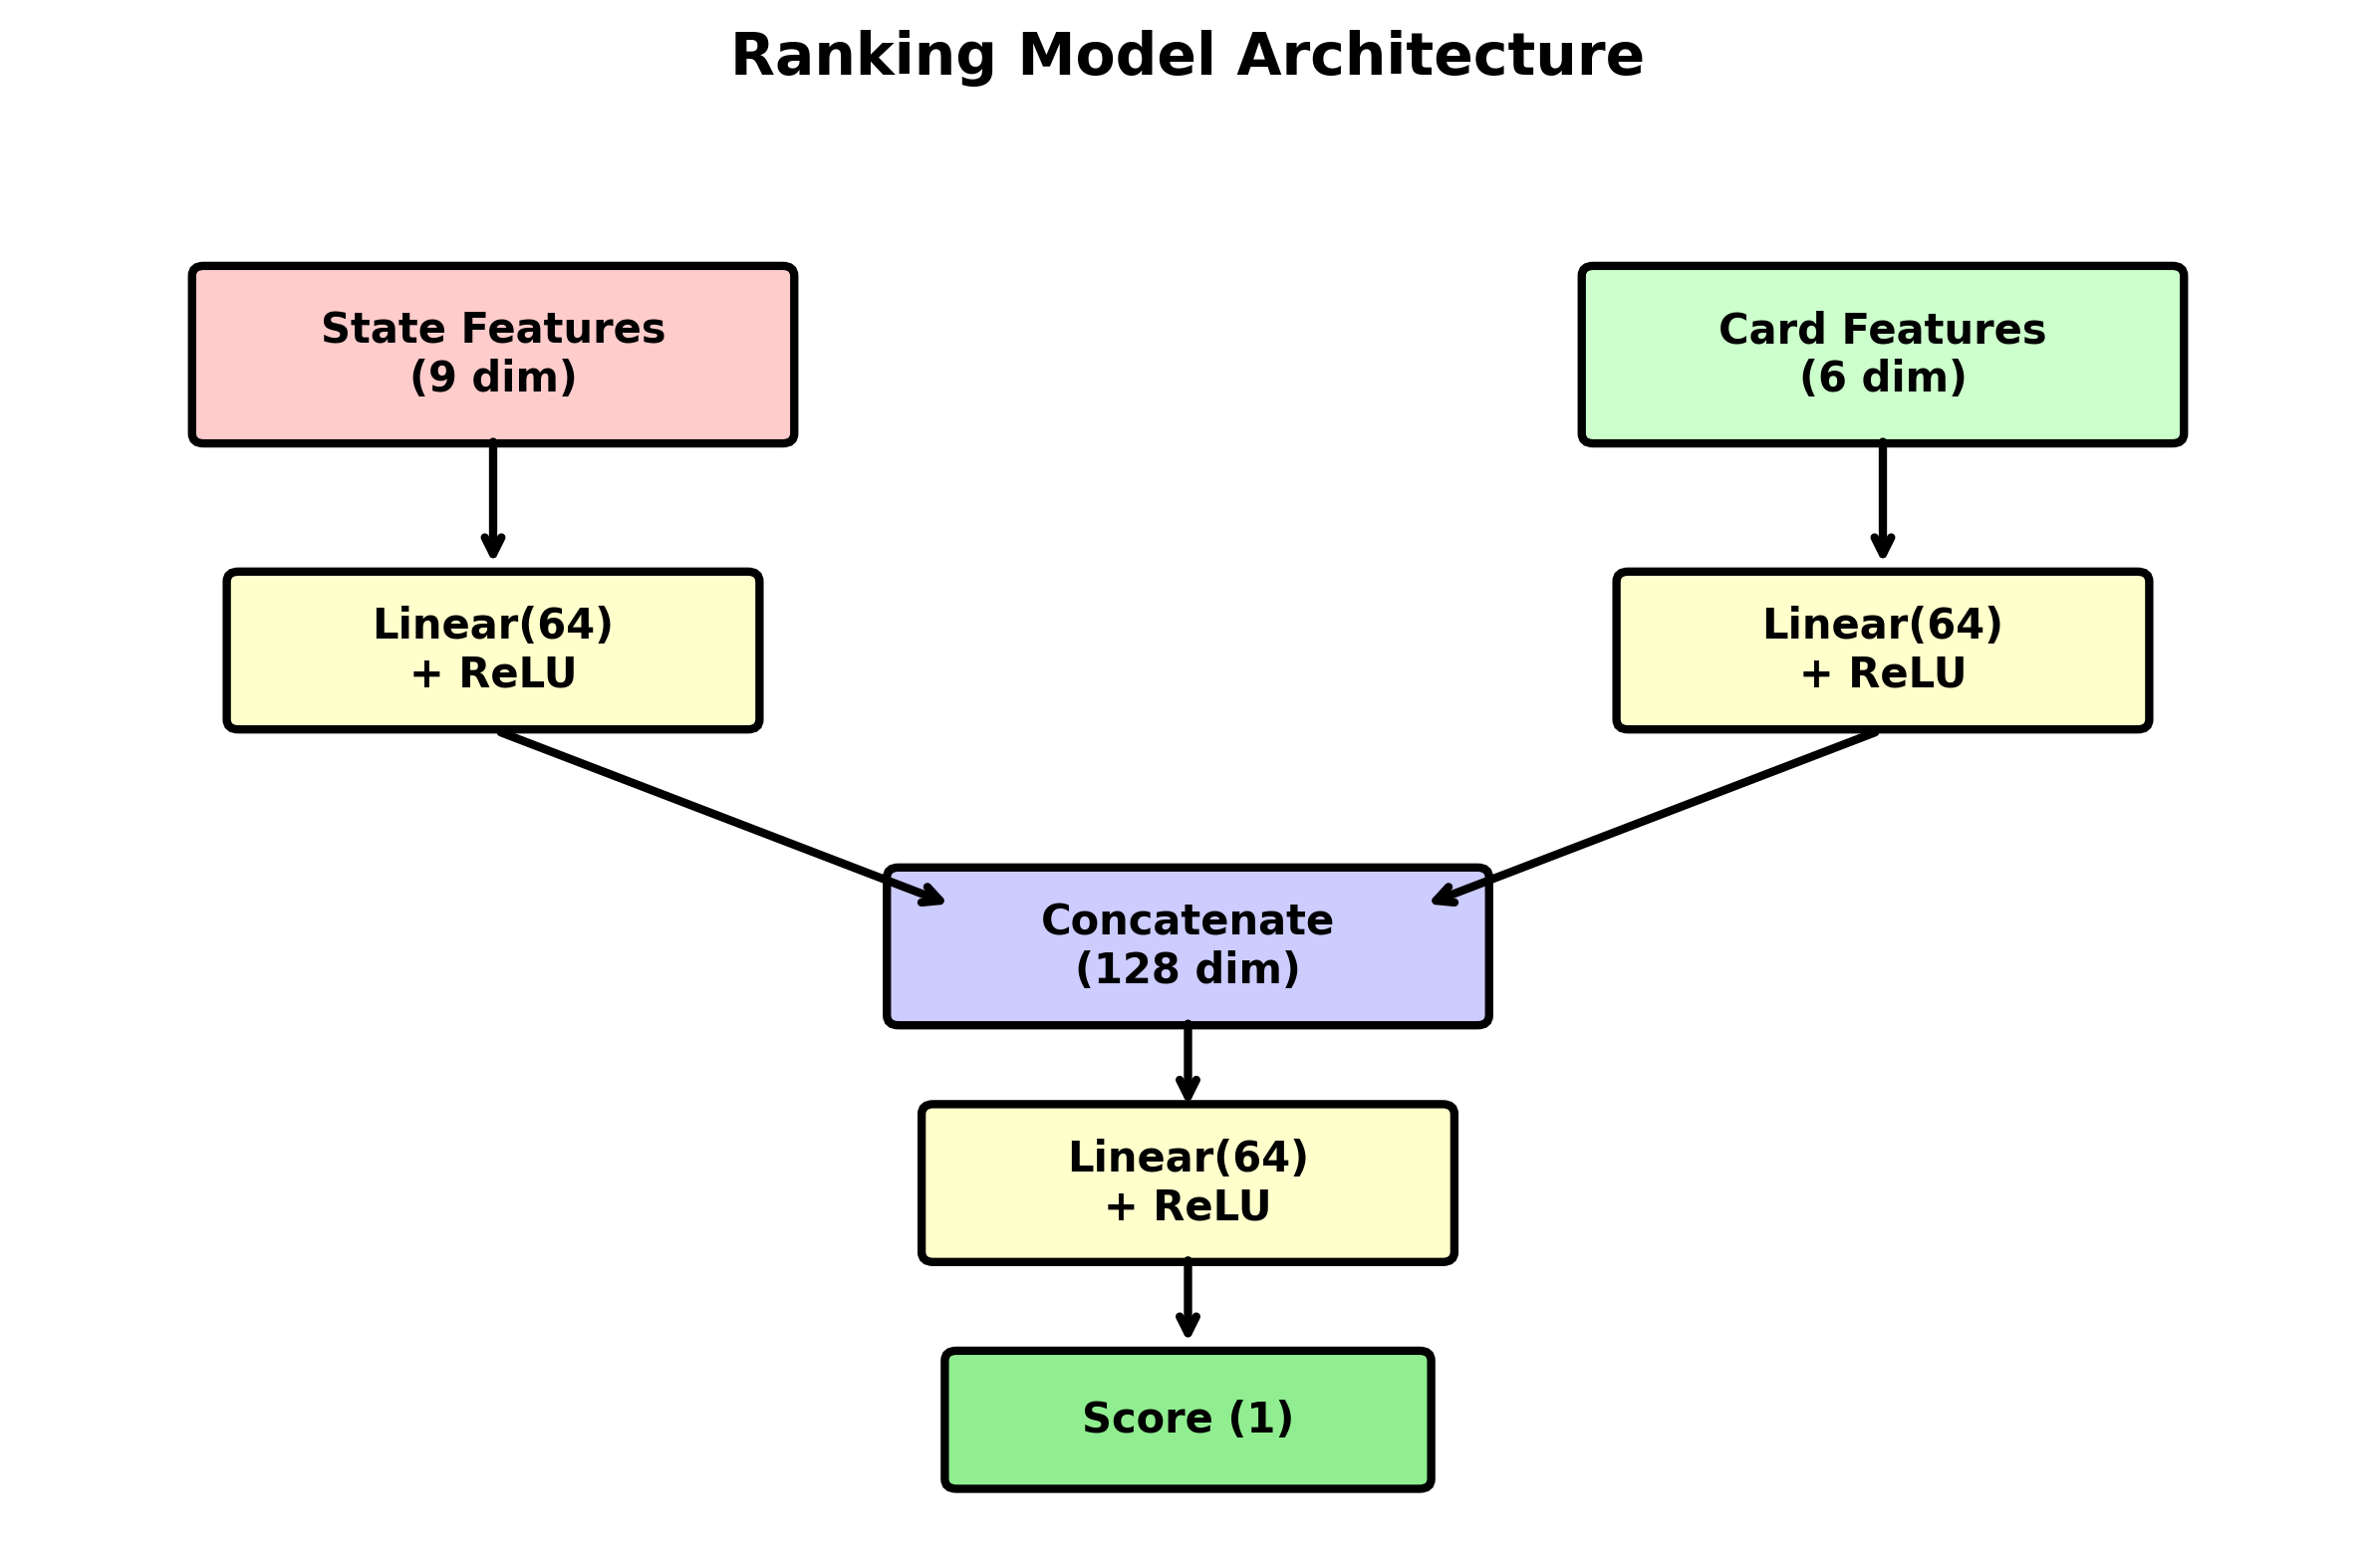
\includegraphics[width=0.9\columnwidth]{ranking_architecture.png}}
\caption{Ranking model neural network architecture. State and card features are processed through independent embedding networks before concatenation and final scoring layers.}
\label{fig:architecture}
\end{figure}

\textbf{State features} (9 dimensions) capture the current game context:
\begin{itemize}
    \item Trick number (normalized to [0, 1])
    \item Is declarer team (binary indicator)
    \item Number of cards played in current trick (0-3)
    \item Number of legal actions available
    \item Count of trump cards remaining in hand
    \item Total point value of cards in hand
    \item Points currently in the trick
    \item Whether trump has been played in the trick
    \item Whether the led suit is trump
\end{itemize}

\textbf{Card features} (6 dimensions) characterize each candidate action:
\begin{itemize}
    \item Is trump card (binary)
    \item Card strength (hierarchical position, normalized)
    \item Point value of the card (normalized)
    \item Whether the card follows the led suit
    \item Whether playing this card would currently win the trick
    \item Relative rank within cards of the same suit in hand
\end{itemize}

The model architecture consists of two parallel branches: a state encoder (Linear(9, 64) + ReLU) and a card encoder (Linear(6, 64) + ReLU). The outputs are concatenated into a 128-dimensional vector, passed through another hidden layer (Linear(128, 64) + ReLU), and finally projected to a scalar score via Linear(64, 1).

\subsection{Training Procedure}

We train the ranking model using margin ranking loss, which encourages the model to score the better action higher than the worse action by at least a margin $m$:

\begin{equation}
\mathcal{L} = \max(0, -y \cdot (f(s, a_{best}) - f(s, a_{worse})) + m)
\end{equation}

where $y = 1$ (indicating $a_{best}$ should score higher), $m = 0.1$ is the margin hyperparameter, and $f(s, a)$ is the ranking model's score for taking action $a$ in state $s$. Training uses the Adam optimizer with learning rate $10^{-3}$ and weight decay $10^{-4}$ for regularization, running for 100 epochs with early stopping based on validation accuracy.

\subsection{Hybrid Agent Decision Procedure}

The hybrid agent (Figure~\ref{fig:hybrid}) combines the reliability of rule-based play with the corrective capability of the learned model through a confidence-thresholded override mechanism:

\begin{enumerate}
    \item Query the rule-based agent for its recommended action $a_{RB}$
    \item Score all legal actions using the trained ranking model
    \item Identify the highest-scoring action according to the model: $a_{best}$
    \item If the score difference exceeds a threshold, $f(s, a_{best}) - f(s, a_{RB}) > t$, play the model's recommendation $a_{best}$; otherwise default to the rule-based choice $a_{RB}$
\end{enumerate}

The threshold $t$ is a critical hyperparameter that controls the trade-off between trusting the learned model and defaulting to the proven rule-based play. Higher thresholds result in fewer overrides (more conservative behavior), while lower thresholds allow more model corrections but risk overriding correct rule-based decisions.

\begin{figure}[htbp]
\centerline{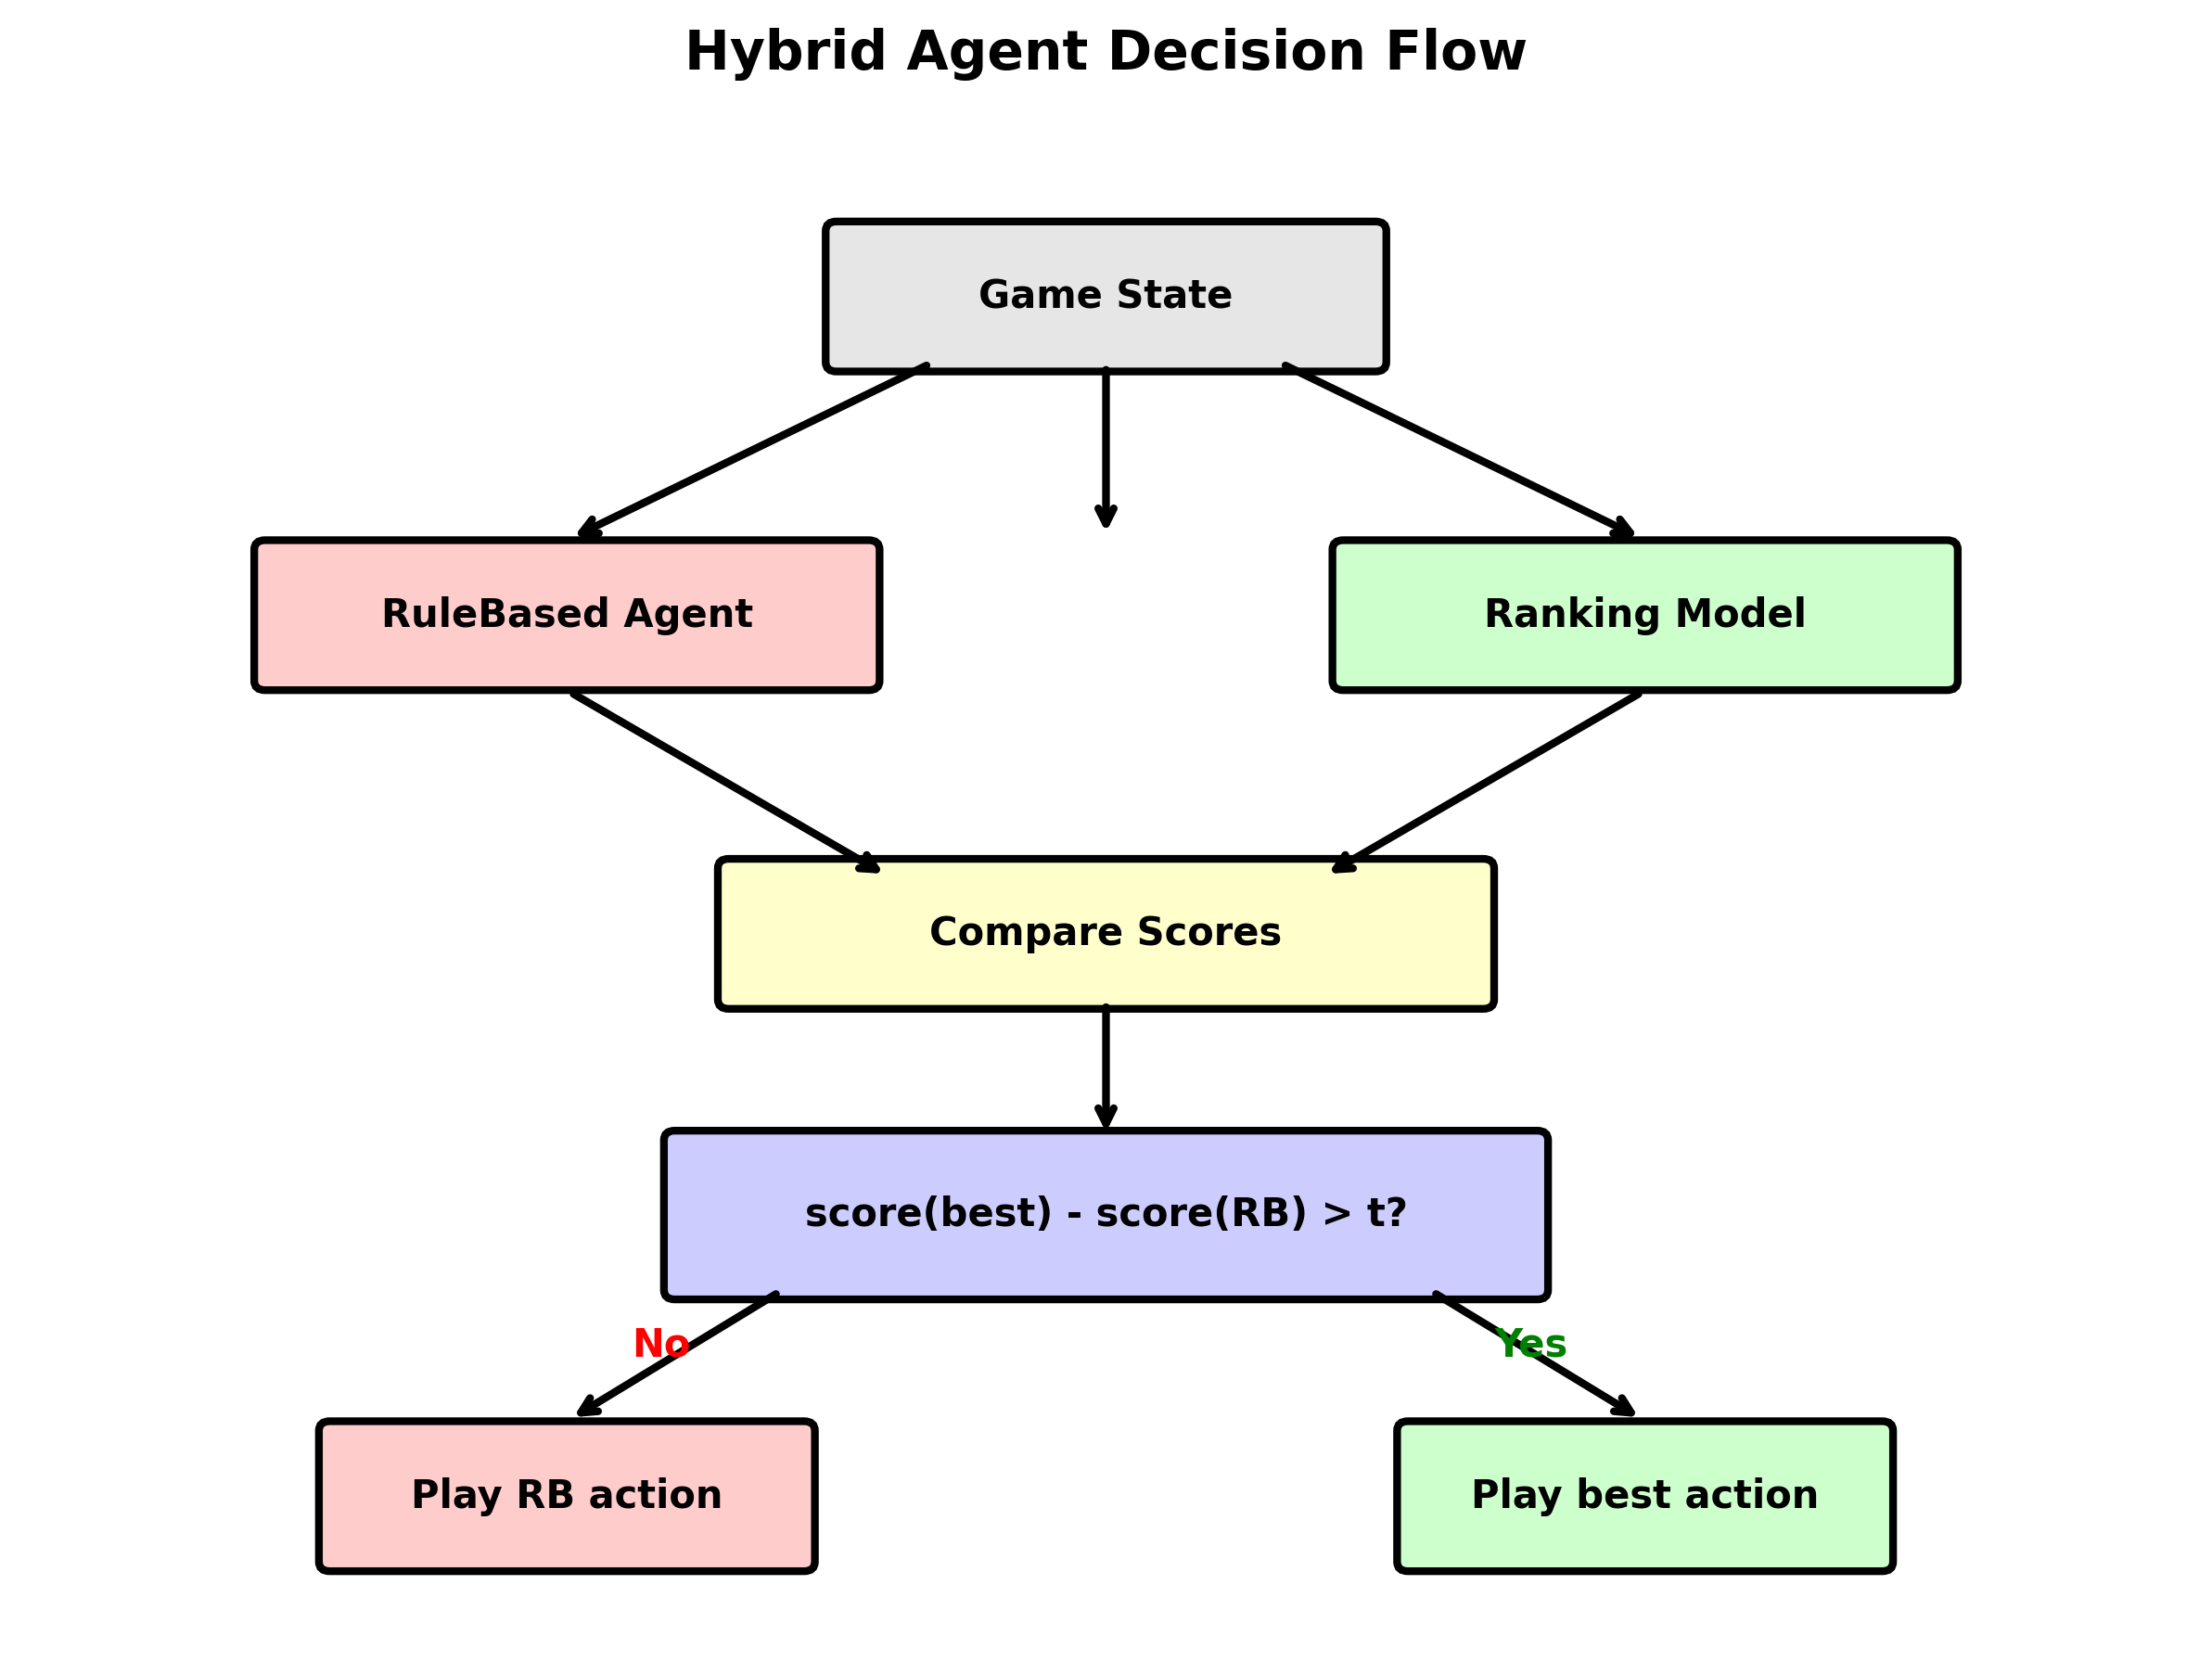
\includegraphics[width=\columnwidth]{hybrid_flow.png}}
\caption{Hybrid agent decision flow diagram. The rule-based action is overridden only when the neural ranking model is confident that a significantly better action exists.}
\label{fig:hybrid}
\end{figure}

\section{Experimental Evaluation}

\subsection{Model Training Results}

The ranking model achieves 68.9\% validation accuracy on held-out pairwise comparisons (Table~\ref{tab:training}), using an 80/20 train/validation split. This represents a substantial improvement over the 50\% random guessing baseline and indicates the model has successfully learned meaningful action preferences from the Monte Carlo oracle data. The relatively modest accuracy (compared to typical classification tasks) reflects the inherent difficulty of the problem and the noise in Monte Carlo estimates, but proves sufficient for improving gameplay.

\begin{table}[htbp]
\caption{Model Training Results}
\begin{center}
\begin{tabular}{lcc}
\toprule
\textbf{Metric} & \textbf{Value} \\
\midrule
Training pairs & 64,333 \\
Validation split & 20\% \\
Final validation accuracy & 68.9\% \\
Training epochs & 100 \\
Best epoch & 60 \\
Model parameters & 12,929 \\
Training time & $\sim$5 minutes \\
\bottomrule
\end{tabular}
\label{tab:training}
\end{center}
\end{table}

\subsection{Override Threshold Analysis}

We evaluated multiple threshold values to find the optimal balance between override frequency and gameplay performance (Figure~\ref{fig:threshold}). This analysis reveals a clear trade-off: too few overrides (high threshold) leaves most rule-based weaknesses unexploited, while too many overrides (low threshold) introduces model errors that degrade performance.

\begin{figure}[htbp]
\centerline{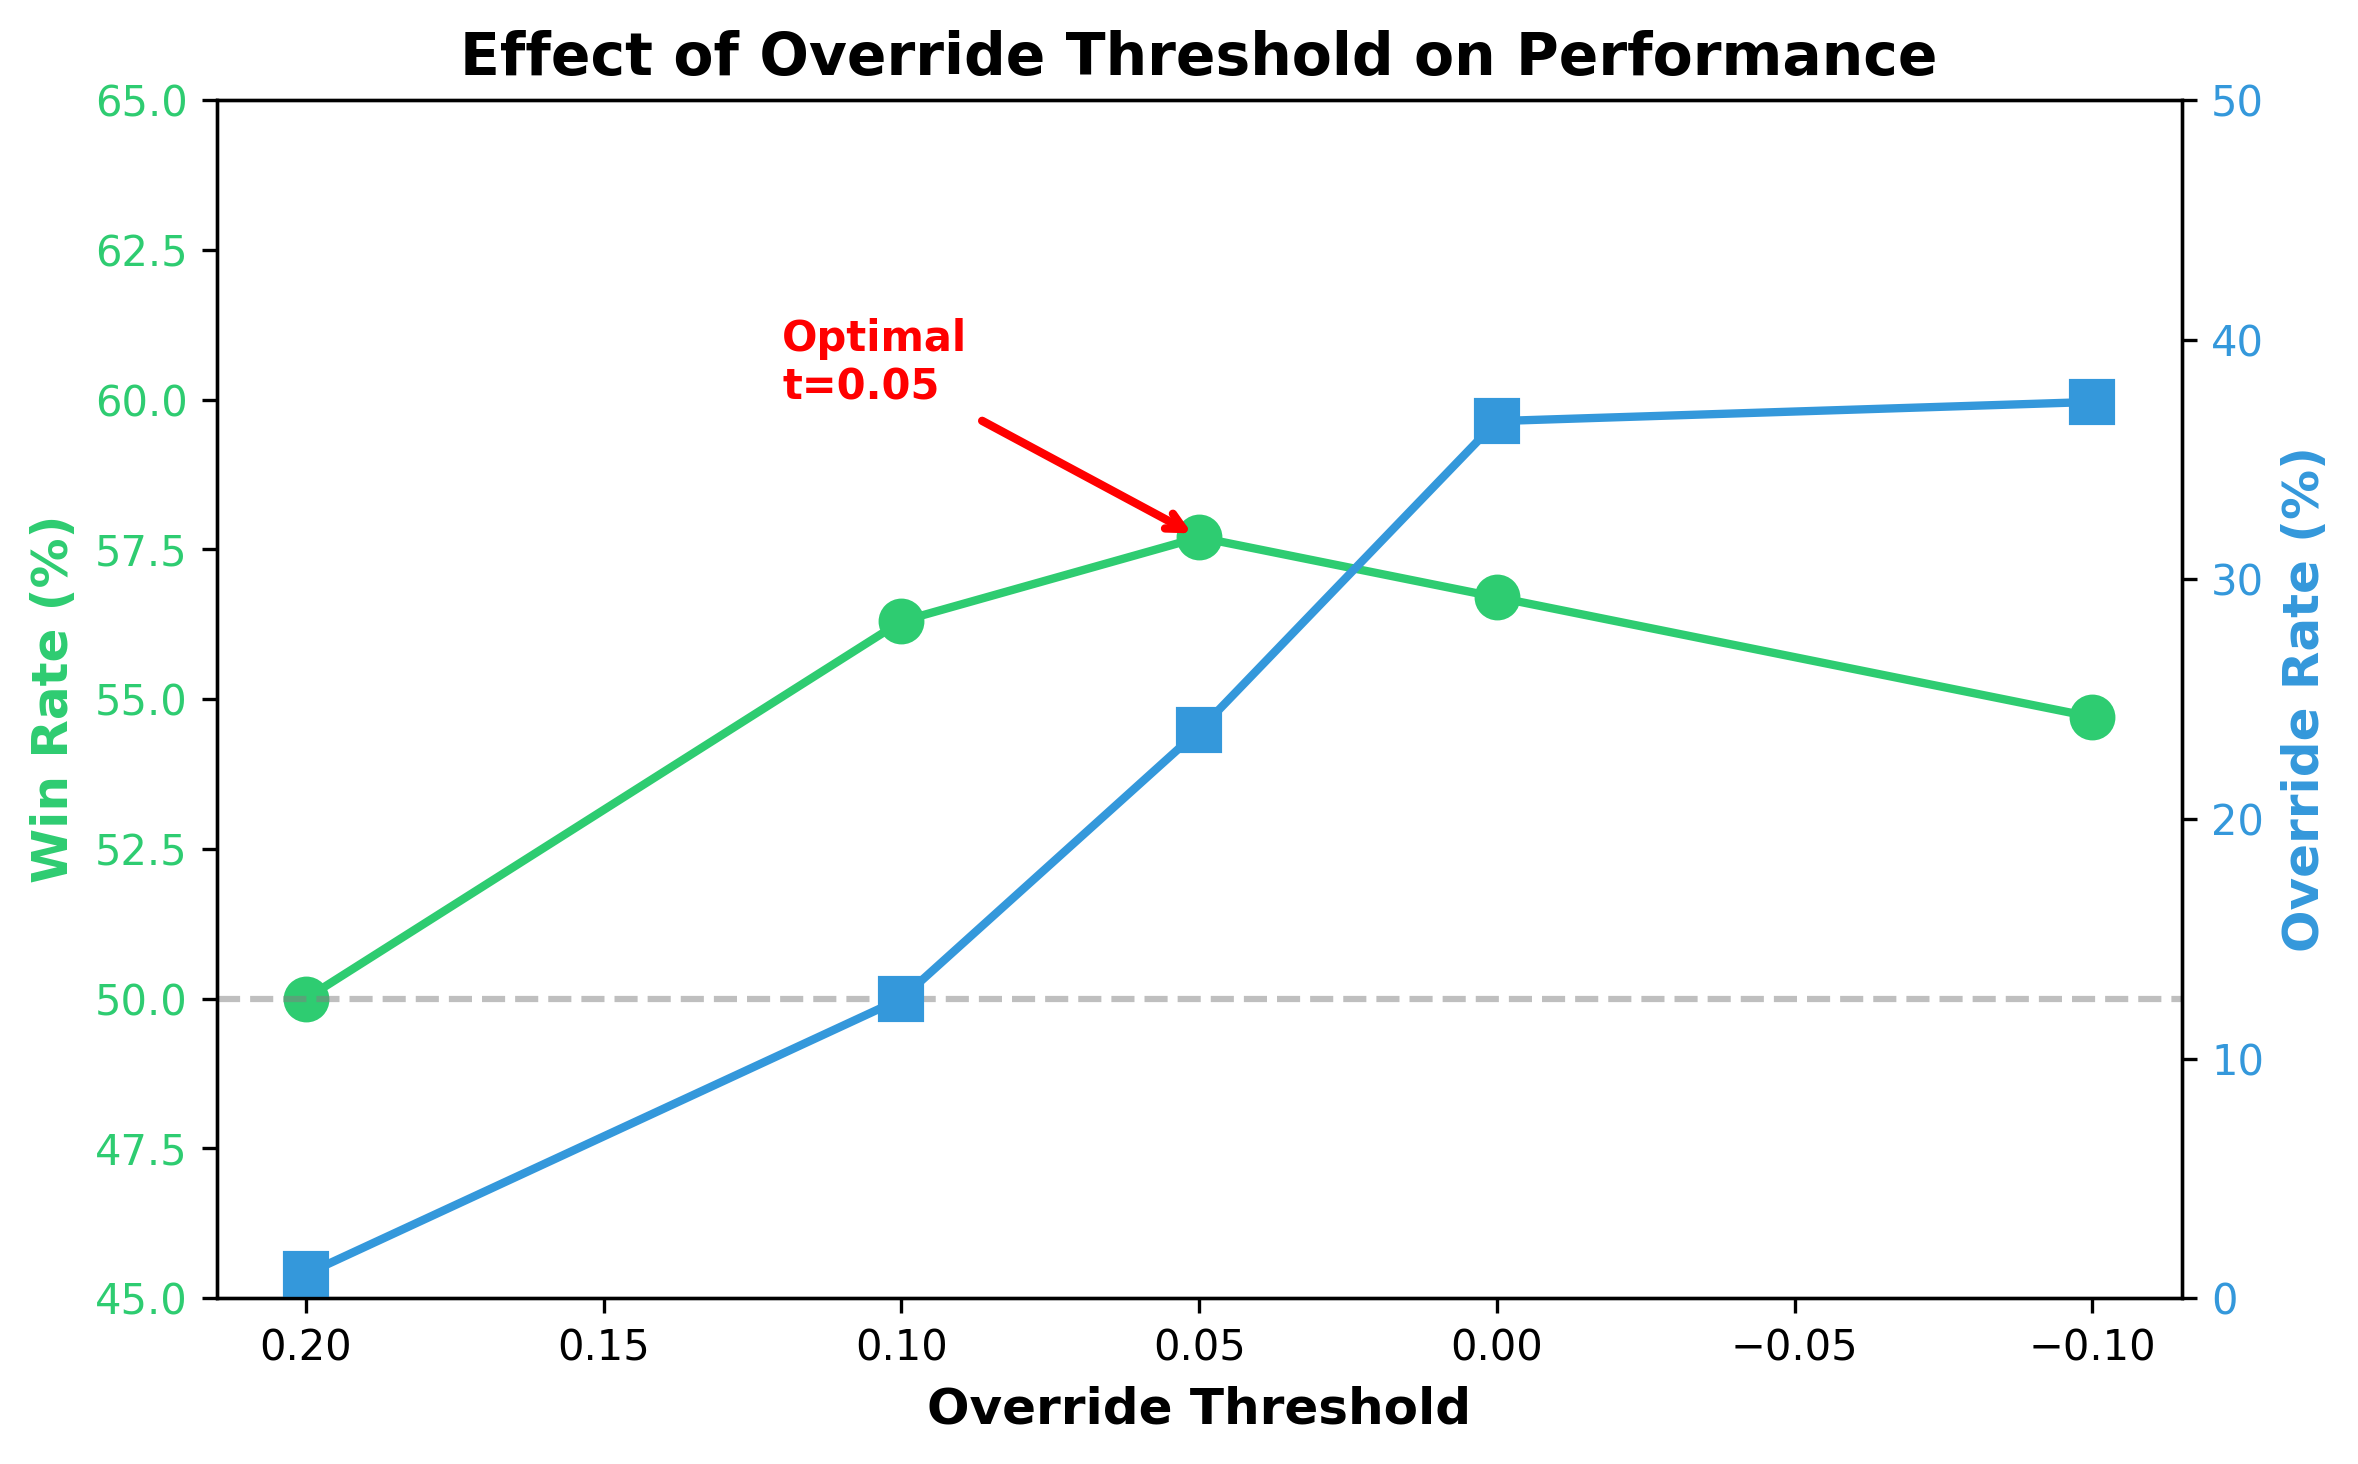
\includegraphics[width=\columnwidth]{threshold_analysis.png}}
\caption{Effect of override threshold on win rate and override frequency. The optimal threshold ($t=0.05$) achieves 57.7\% win rate with 23.7\% override rate, representing the best trade-off between correction and caution.}
\label{fig:threshold}
\end{figure}

\begin{table}[htbp]
\caption{Performance vs. Override Threshold}
\begin{center}
\begin{tabular}{cccc}
\toprule
\textbf{Threshold} & \textbf{Win Rate} & \textbf{Override Rate} & \textbf{Games} \\
\midrule
0.20 & 50.0\% & 1.0\% & 300 \\
0.10 & 56.3\% & 12.5\% & 1000 \\
\textbf{0.05} & \textbf{57.7\%} & \textbf{23.7\%} & 1000 \\
0.00 & 56.7\% & 36.6\% & 300 \\
-0.10 & 54.7\% & 37.4\% & 300 \\
\bottomrule
\end{tabular}
\label{tab:threshold}
\end{center}
\end{table}

The optimal threshold $t = 0.05$ achieves a 57.7\% win rate with a 23.7\% override rate, meaning the model corrects approximately one in four rule-based decisions. Higher thresholds are too conservative and rarely override, leaving exploitable weaknesses intact. Lower thresholds override too frequently, introducing errors when the model incorrectly believes it has found a better action.

\subsection{Comprehensive Algorithm Comparison}

Figure~\ref{fig:comparison} and Table~\ref{tab:comparison} compare all evaluated approaches against the rule-based baseline, providing a complete picture of our exploration.

\begin{figure}[htbp]
\centerline{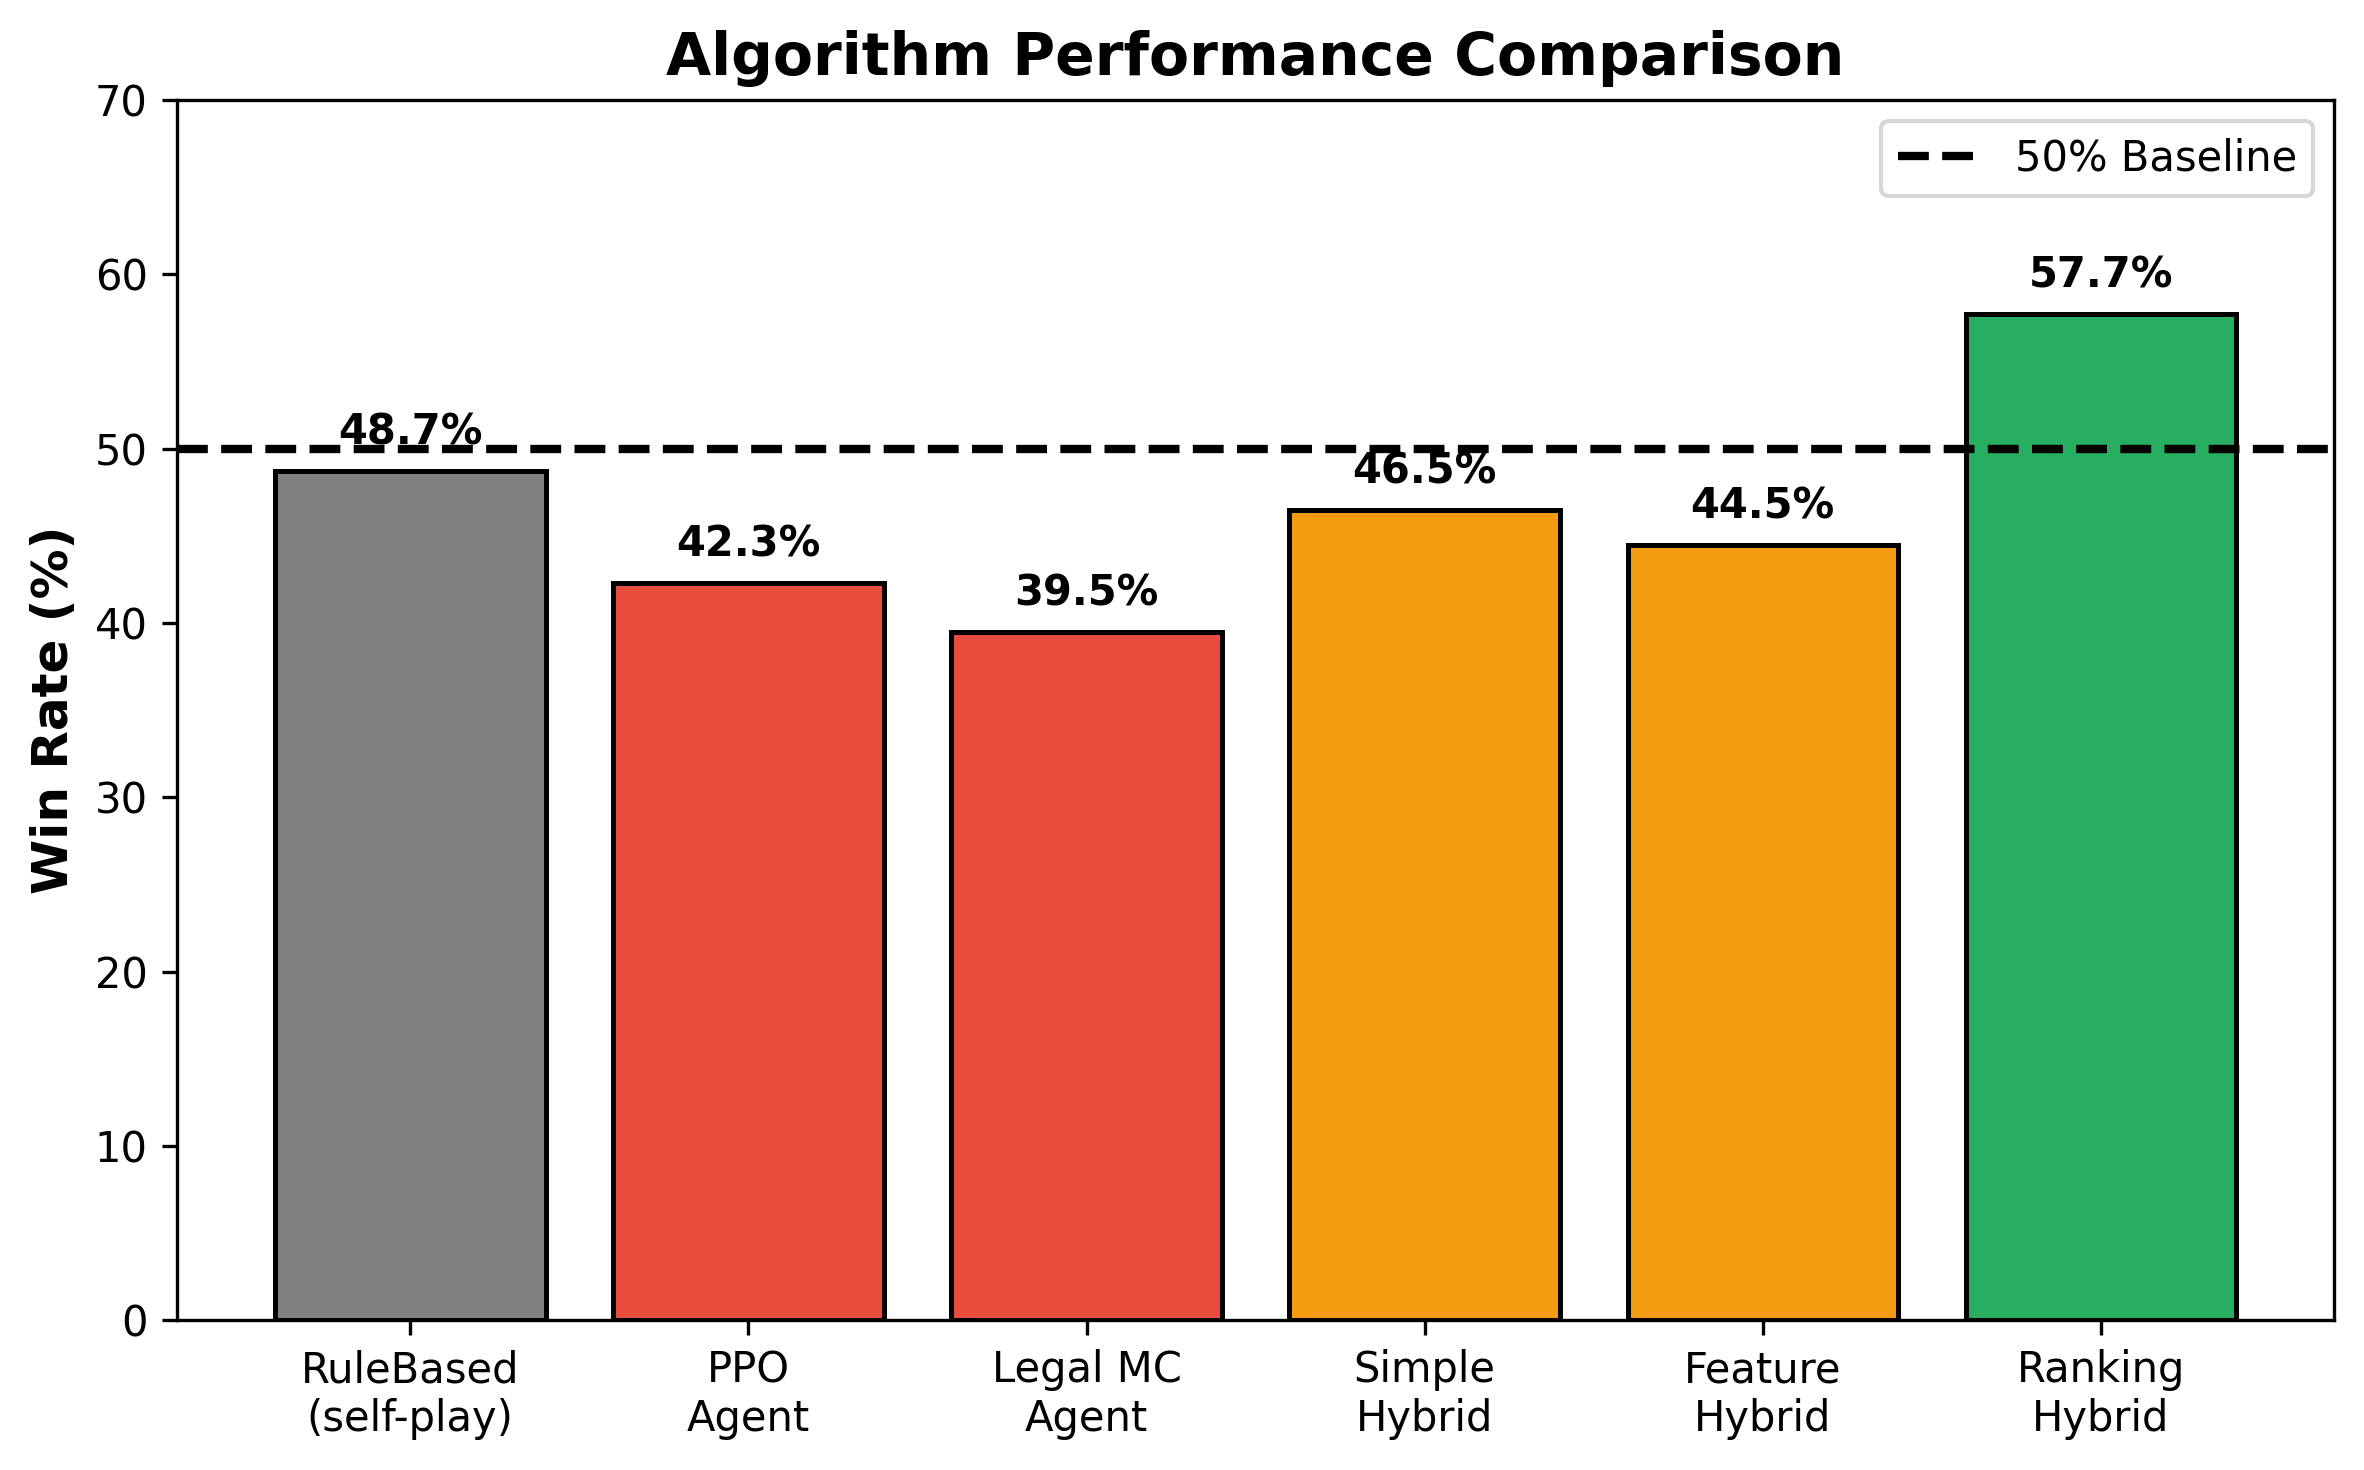
\includegraphics[width=\columnwidth]{algorithm_comparison.png}}
\caption{Win rate comparison of different AI approaches against the rule-based opponent. Only the ranking hybrid method exceeds the 50\% baseline, demonstrating the importance of our pairwise ranking and confidence-thresholded override approach.}
\label{fig:comparison}
\end{figure}

\begin{table}[htbp]
\caption{Comprehensive Algorithm Comparison}
\begin{center}
\begin{tabular}{lcc}
\toprule
\textbf{Algorithm} & \textbf{Win Rate} & \textbf{vs Baseline} \\
\midrule
RuleBased (self-play) & 48.7\% & — \\
PPO Agent & 42.3\% & -6.4\% \\
Legal MC Agent & 39.5\% & -9.2\% \\
Simple Hybrid (Lookup) & 46.5\% & -2.2\% \\
Feature Hybrid & 44.5\% & -4.2\% \\
\textbf{Ranking Hybrid (Ours)} & \textbf{57.7\%} & \textbf{+9.0\%} \\
\bottomrule
\end{tabular}
\label{tab:comparison}
\end{center}
\end{table}

The ranking hybrid is the only approach to exceed the 50\% baseline, achieving a commanding 57.7\% win rate. This represents a 9 percentage point improvement over equal play and demonstrates the effectiveness of our hybrid approach.

\subsection{Statistical Significance Analysis}

Over 1,000 games, the ranking hybrid won 577 games (57.7\%). Using a one-proportion z-test against the null hypothesis of a 50\% win rate (which would indicate no improvement over the baseline):

\begin{equation}
z = \frac{0.577 - 0.50}{\sqrt{0.50 \times 0.50 / 1000}} = 4.87
\end{equation}

This yields $p < 0.0001$, providing overwhelming statistical evidence that the improvement is genuine and not attributable to random variance. The 95\% confidence interval for the true win rate is [54.6\%, 60.8\%], entirely above the 50\% baseline.

\section{Analysis and Discussion}

\subsection{Characterizing Override Patterns}

Analysis of override patterns reveals that the ranking model most frequently corrects rule-based decisions in specific, identifiable situations. Understanding these patterns provides insight into the weaknesses of the heuristic approach and validates that the model has learned meaningful corrections:

\begin{itemize}
    \item \textbf{Late-game point management}: In tricks 6-8, when point totals are close to the critical 61-point threshold, the model frequently overrides conservative rule-based play with more aggressive or defensive moves appropriate to the margin
    \item \textbf{Trump conservation}: The model identifies situations where the rule-based agent plays high trumps unnecessarily, preserving them for more impactful moments
    \item \textbf{Partner coordination}: When defending, the model recognizes opportunities to support partner plays that the rule-based heuristics miss
    \item \textbf{Sacrifice plays}: Occasionally, the model recommends sacrificing a trick with low points to set up winning a subsequent high-point trick
\end{itemize}

These override categories align with known areas where heuristic Schafkopf players struggle, providing face validity for our learned corrections.

\subsection{Computational Efficiency}

A significant practical advantage of our approach is its computational efficiency. Unlike deep reinforcement learning methods that require millions of training steps and hours of compute time, our hybrid method:
\begin{itemize}
    \item Trains in approximately 5 minutes on a standard CPU
    \item Requires no GPU acceleration
    \item Uses a compact model with fewer than 13,000 parameters
    \item Maintains real-time inference speed (sub-millisecond per decision)
\end{itemize}

This efficiency makes the approach practical for deployment and accessible to researchers without access to extensive computational resources.

\subsection{Limitations and Future Directions}

Our approach has several limitations that suggest directions for future research:

\begin{itemize}
    \item \textbf{Oracle quality}: Monte Carlo estimates using only 100 rollouts have high variance; increasing the rollout count or using more sophisticated value estimation could improve training data quality
    \item \textbf{Game mode generalization}: We evaluated only the Sauspiel mode; other Schafkopf modes (Solo, Wenz, Geier) have different dynamics and may require mode-specific models or multi-task learning
    \item \textbf{Opponent adaptation}: The hybrid agent was trained against the same rule-based agent it plays against; performance against human players or different AI systems remains to be evaluated
    \item \textbf{Exploration of architecture}: The relatively simple neural network architecture leaves room for experimentation with attention mechanisms, transformers, or other modern architectures
\end{itemize}

\section{Conclusion}

We presented a novel hybrid AI approach for Schafkopf that combines traditional rule-based play with a learned neural ranking model, achieving a 57.7\% win rate against a strong rule-based baseline—a statistically significant 9 percentage point improvement. Our key contributions and findings include:

\begin{enumerate}
    \item Demonstrating that learning to rank actions through pairwise comparisons is more effective than learning to predict absolute action values, confirming the power of the learning-to-rank paradigm for game playing
    \item Showing that selective override with confidence thresholding outperforms both pure learning approaches (which lack sufficient training signal) and pure rule-based approaches (which contain exploitable weaknesses)
    \item Providing a lightweight and computationally efficient methodology applicable to other domains where strong heuristic solutions already exist but contain room for improvement
    \item Contributing an open-source Schafkopf environment and trained models to facilitate future research on this underexplored game
\end{enumerate}

The broader implication of our work is that in domains where expert-designed heuristics exist, the most effective learning approach may not be to replace these heuristics entirely, but rather to learn when and how to improve upon them. This hybrid philosophy—trusting existing solutions while learning targeted corrections—offers a practical path to AI improvement that is both effective and computationally accessible.

Future work could extend this approach to other Schafkopf game modes, incorporate opponent modeling to adapt corrections dynamically, or apply the methodology to other trick-taking card games where rule-based agents remain competitive. The success of our pairwise ranking approach also suggests potential applications beyond card games, in any domain where action selection from a small set of candidates is required.

\section*{Acknowledgment}

We thank the PettingZoo developers for their multi-agent environment framework.

\begin{thebibliography}{00}

\bibitem{billings2002challenge}
D. Billings, A. Davidson, J. Schaeffer, and D. Szafron, ``The challenge of poker,'' \textit{Artificial Intelligence}, vol. 134, no. 1-2, pp. 201--240, 2002.

\bibitem{tian2020joint}
Z. Tian, Y. Liu, H. Li, and Q. Yang, ``Joint policy search for multi-agent collaboration with imperfect information,'' \textit{NeurIPS}, 2020.

\bibitem{doppelkopf2019}
S. Kupferschmid and H. Helmert, ``A Skat player based on Monte Carlo simulation,'' \textit{Computers and Games}, pp. 135--147, 2006.

\bibitem{silver2016mastering}
D. Silver et al., ``Mastering the game of Go with deep neural networks and tree search,'' \textit{Nature}, vol. 529, no. 7587, pp. 484--489, 2016.

\bibitem{silver2017mastering}
D. Silver et al., ``Mastering Chess and Shogi by self-play with a general reinforcement learning algorithm,'' \textit{arXiv preprint arXiv:1712.01815}, 2017.

\bibitem{brown2019superhuman}
N. Brown and T. Sandholm, ``Superhuman AI for multiplayer poker,'' \textit{Science}, vol. 365, no. 6456, pp. 885--890, 2019.

\bibitem{kupferschmid2006skat}
S. Kupferschmid and H. Helmert, ``A Skat player based on Monte Carlo simulation,'' \textit{Computers and Games}, 2006.

\bibitem{ginsberg2001gib}
M. L. Ginsberg, ``GIB: Imperfect information in a computationally challenging game,'' \textit{Journal of Artificial Intelligence Research}, vol. 14, pp. 303--358, 2001.

\bibitem{burges2010ranknet}
C. Burges et al., ``From RankNet to LambdaRank to LambdaMART: An overview,'' \textit{Learning}, vol. 11, no. 23-581, p. 81, 2010.

\bibitem{rendle2012bpr}
S. Rendle, C. Freudenthaler, Z. Gantner, and L. Schmidt-Thieme, ``BPR: Bayesian personalized ranking from implicit feedback,'' \textit{UAI}, 2009.

\bibitem{schulman2017proximal}
J. Schulman, F. Wolski, P. Dhariwal, A. Radford, and O. Klimov, ``Proximal policy optimization algorithms,'' \textit{arXiv preprint arXiv:1707.06347}, 2017.

\bibitem{terry2021pettingzoo}
J. Terry et al., ``PettingZoo: Gym for multi-agent reinforcement learning,'' \textit{NeurIPS}, 2021.

\end{thebibliography}

\end{document}
